\documentclass[a4paper,11pt]{article}
\usepackage{a4wide}
\usepackage[ansinew]{inputenc}
\usepackage{graphicx}
\usepackage{bm}
\usepackage{natbib}
\usepackage{longtable}
\usepackage{rotating}
\usepackage{pdflscape}
%\usepackage{pdfdraftcopy}


%\usepackage{jurabib}
   %\jurabibsetup{  
     %authorformat=and  
    % commabeforerest,  
    % titleformat=colonsep,  
    % bibformat=tabular  
   %}  

\usepackage[bookmarks=true, bookmarksopen=true,
                bookmarksnumbered=true, colorlinks,citecolor = blue,
                filecolor=blue, linkcolor=blue, urlcolor=blue,
                plainpages=false,hyperindex=true]{hyperref}
\hypersetup{
        pdftitle={},
        pdfauthor={Anton Burger and Robert Ferstl},
        pdfsubject={},
        pdfkeywords={},
        pdfcreator={},
        pdfproducer={}
     }

%\usepackage{natbib}
%\usepackage{dingbat}
\usepackage{amssymb,amsmath,amstext}
%\usepackage{manfnt}

\setlength{\parindent}{0.0cm}                      % Absatzeinr�ckungen
\setlength{\parskip}{1.5ex plus 0.5ex minus 0.5ex} % Absatzabst�nde
%\renewcommand{\arraystretch}{1.5}                 % Zeilenabstand in Tabellen


\begin{document}
\title{Generation Capacity Investment in Electricity Markets \\ in an Oligopolistic, Dynamic and Stochastic Framework\\\vspace{0.3cm}\emph{Draft version}\thanks{Please do not cite without consulting the authors.}}
\author{Anton Burger\thanks{\href{http://www.wu-wien.ac.at/regulierung}{Institute for Regulatory Economics, Vienna University of Economics and Business Administration,} \href{mailto:anton.burger@wu-wien.ac.at}{anton.burger@wu-wien.ac.at}}\hspace{1cm} Robert Ferstl\thanks{\href{http://www-finanzierung.uni-regensburg.de/}{Department of Finance, University of Regensburg,} \href{mailto:robert.ferstl@wiwi.uni-regensburg.de}{robert.ferstl@wiwi.uni-regensburg.de}}}
\maketitle
\abstract{
The paper discusses game theoretic models for generation capacity investment decisions in a deregulated electricity market. The possible problem formulations involve open-loop, closed-loop and $S$-adapted Cournot equilibria. We present an example of an S-adapted Cournot equilibrium, which we apply to the German electricity market. Investment decisions derived by this dynamic oligopoly model are then compared to what the perfect competition result in an otherwise unchanged setup would be. We conclude that there seems to be a problem with underinvestment and technology mix in the current market structure.
\\
\\


\textbf{Keywords:} Electricity markets, Investment decisions, Stochastic oligopoly model, Sample path optimization, Stochastic programming
\\
\\
\textbf{JEL Codes:} D43, L51
}

\section{Introduction}

In this paper we will build a model for generation capacity investment under uncertainty. We consider a deregulated electricity market, where typically several large players act on market leading to an oligopoly situation. There is not much literature which directly deals with the question of  generation capacity investments. Recent works are \cite{Chuang2001}, \cite{Ventosa2002}, \cite{Chaton2003}, \cite{Hogendorn2003}, \cite{Pineau2003}, \cite{Ehrenmann2004}. \cite{Murphy2005}, \cite{Kiesling2007}, \cite{Pineau2007}.


Cournot is more flexible and better computational tractability.

\subsection{The Austrian electricity market}

approximately half page about Austrian electricity market: total consumption, major players, progress of deregulation, major generation technologies, competitive fringe, types of trades in the market


\subsection{Stochastic oligopoly models}

\textbf{References:} \cite{Salant1982, Wolf1997, Haurie2002, Pineau2003, Murto2004}\\


The $S$-adapted information structure was introduced by \cite{Haurie1990}.
$S$-adapted structure is similar to the open-loop case, except that the strategies of the players adapt to the sample path of the stochastic variable \citep[see][pg. 128]{Pineau2003}.

\cite{Haurie2002} developed an approximation method with variational inequalities for $S$-adapted oligopoly equilibria. It can be used with any discrete state process that can be represented as an event tree can be used as description of the random disturbances.

\cite{Murto2004} solves the game with feedback information structure.

\subsection{Short-term assumption for decision variables}

Cournot, Bertrand, SFE


In theory, the output of a competitive generation market is equal to the output of a regulated system with a central planner that minimizes investment plus operating costs to meet demand (Green, 2000), see \citep[see][pg. 111]{Rothwell2003}.

Papers with focus investment problem: \cite{Pineau2003}, \cite{Murphy2005}, \cite{Genc2007}, \cite{Kiesling2007}, \cite{Barmack2007}, \cite{Sauma2006}

Market simulation: \cite{Torre2003}, \cite{Valenzuela2007}, \cite{Hobbs2001},\cite{Otero-Novas2000}

General review paper: \cite{Neuhoff2005}, \cite{Ventosa2005}, \cite{Kahn1998}

%%% Local Variables: 
%%% mode: latex
%%% TeX-master: "../emarket_simulation"
%%% End: 

%\section{Strategic capacity investment decisions under imperfect competition}

\subsection{Cournot solution}

\subsection{Dynamic games and information structures}


\section{Data}

The German electricity market was liberalized in 1998 and is the largest in Europe with a gross production of of 633.2 TWh in 2006 \citep{IEA2007}. More than half of the power is generated with coal, other major sources are nuclear and gas. The German power market is dominated by a few large players (E.ON, RWE, EnBW, Vattenfall). These firms are both transmission system operators and own 90\% of total generation capacity. \cite{Brunekreeft2006} report values for Herfindahl Hirschman Index (HHI)\footnote{This is a common measure of market power and is calculated as sum of the squared market shares in an industry.} of over 2000. Electricity distribution is organized by approximately 900 communal distributors. The German energy market regulator  \emph{Bundesnetzagentur} was installed in 2005. Germany decided on a phase-out of nuclear power generation by 2020. The \emph{German Energy Agency} estimates that investments in generation capacity of up to 40,000 MW will be necessary, see Fig. \ref{fig:nuclear}.

\begin{figure}[htb]
  \centering
\caption{Estimated nuclear power capacity, 2007 to 2023}
  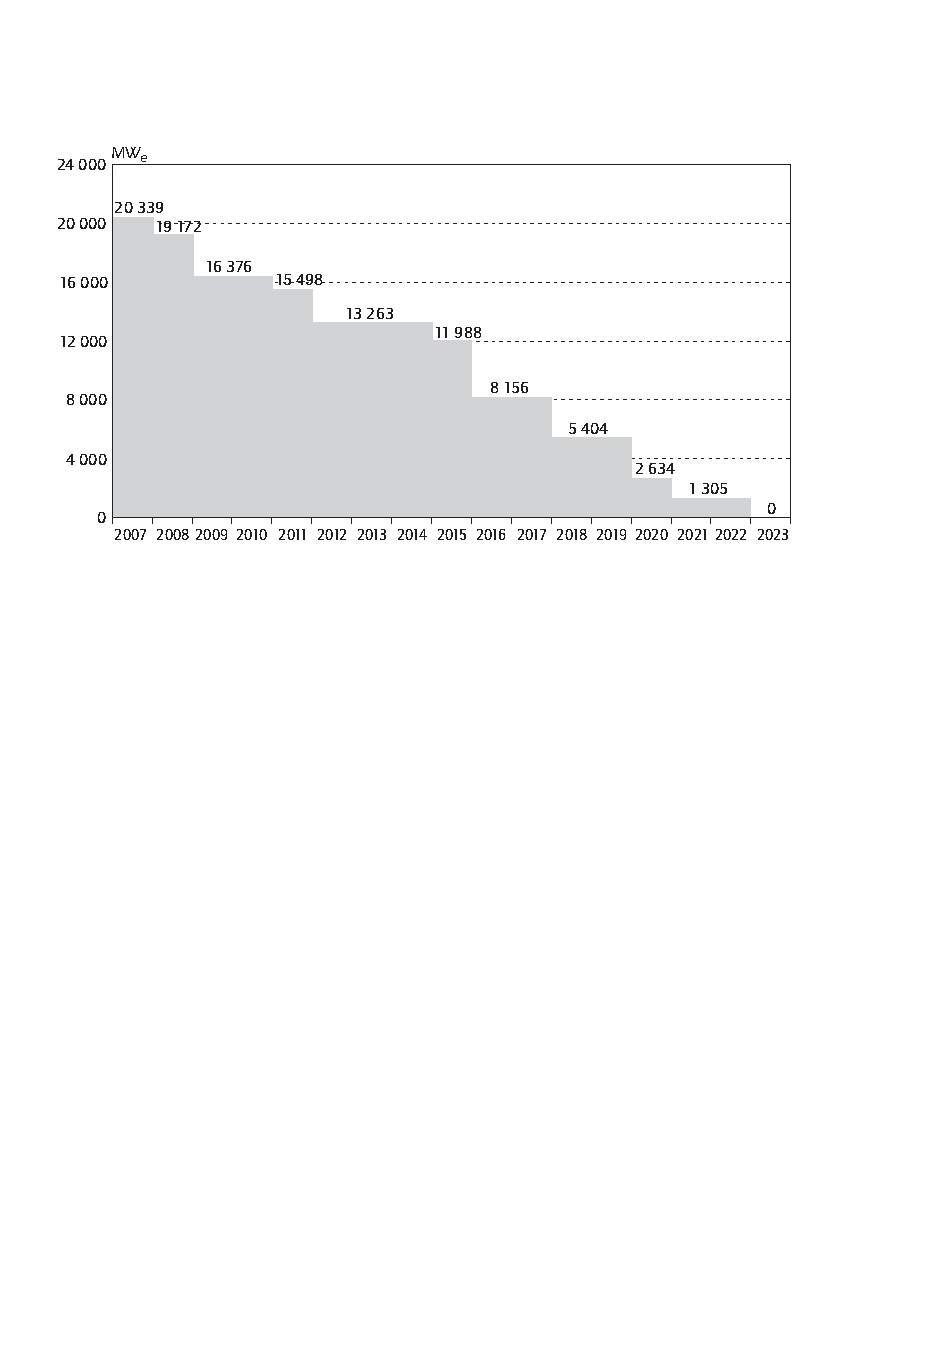
\includegraphics[width=.7\textwidth]{germandata/nuclear.pdf}
  \label{fig:nuclear}
\\
 \scriptsize Source: \cite{IEA2007a}
\end{figure}

The capacities of the four major electricity generators can be found in Tab. \ref{tab:majorcapacities}.

\begin{table}[htb]
\centering
\scriptsize
\caption{Installed capacities in MW of major players in Germany}
\vspace{0.3cm}
\begin{tabular}[htb]{crrrrrrrrr}
\hline
           &      Hydro &    Nuclear &  Soft coal &  Hard coal &        Gas &        Oil &     Pumped \\
\hline\hline
       RWE &        741 &       5499 &      10554 &       7249 &       4297 &        188 &        793 \\

      E.ON &       1320 &       8473 &       1425 &       9461 &       3808 &       1779 &       1110 \\

Vattenfall &          9 &       1421 &       6932 &       1729 &        870 &       1429 &       2883 \\

      EnBW &        447 &       4272 &        453 &       3288 &       1083 &        617 &        368 \\
\hline
\end{tabular} 
\label{tab:majorcapacities}
\\
\vspace{0.3cm}
\scriptsize Source: \cite{Ellersdorfer2005}
\end{table}

%Figure \ref{fig:investcosts} contains investment costs for different technologies.

%\begin{figure}[htb]
%  \centering
%\caption{Levelised costs for generation units starting commercial operation in 2015}
%  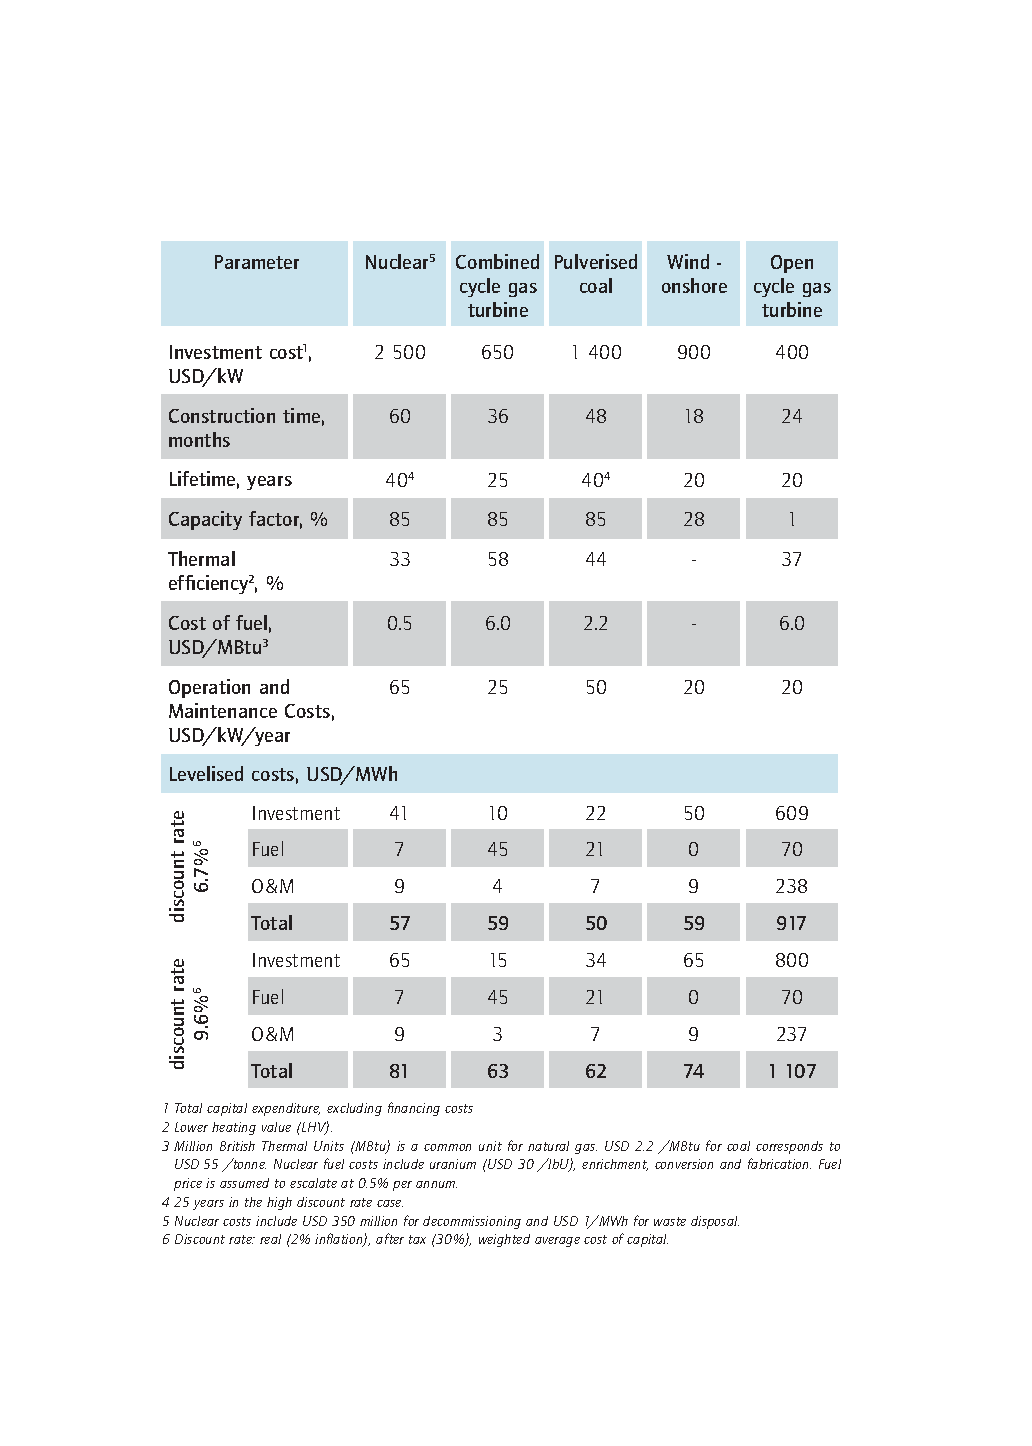
\includegraphics[width=.5\textwidth]{germandata/investmentcosts.pdf}
%  \label{fig:investcosts}
%\\
% \scriptsize Source: \cite{IEA2007c}
%\end{figure}

The major stake of electricity trading is done in OTC markets for which it is hard to obtain data. Exchange prices from the EEX can be used as a good approximation. We see the expected positive relationship when comparing the exchange prices to the actual electricity demand per hour.

\begin{figure}[htb]
  \centering
\caption{Price-quantity relationship}
  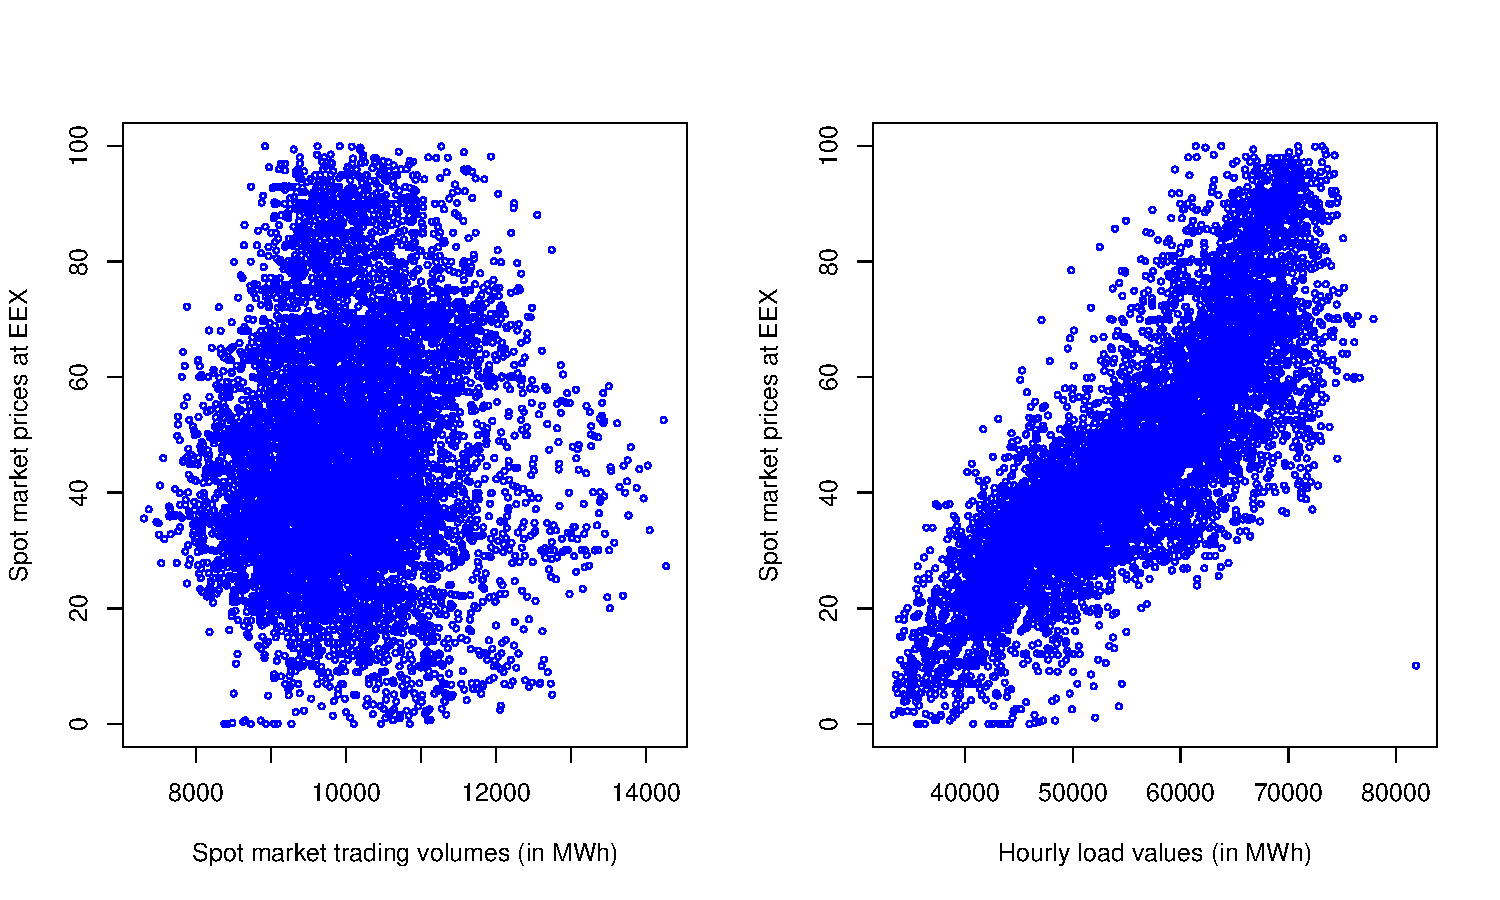
\includegraphics[width=.8\textwidth]{germandata/pricequant.pdf}
  \label{fig:investcosts}
\\
 \scriptsize Source: EEX, UCTE
\end{figure}

To account for different states of the market we separated the price-quantity combinations which occurred within a year by prices. As can be seen in Table \ref{tab:demand}, markets with extremely high prices occur only seldom and prices between 20 and 40 are most common. For each of the six states in which the market might be we created linear demand functions based on average prices and quantities in these states. Note that in order to account for price spikes we model the high-price end of the market quite accurately. To construct demand curves, \cite{Neuhoff2005} use a demand elasticity of 0.1, whereby \cite{Genc2007} argue that 0.2 is more commonly used to simulate the electricity market. As we have a more long run focus we decided to use 0.2 as in the long run, elasticity is higher. It might be argued, that in an electricity market, there is no elasticity anyway as maybe only a very few industrial clients reduce their demand as prices rise. Responding to this, \cite{Bushnell2003} notes that imports and exports provide some elasticity.

\begin{table}[htb]
\centering
\caption{Market segments}
\vspace{0.3cm}
\begin{tabular}{lllll}
\hline
 & \multicolumn{1}{c}{Occupancy} & \multicolumn{1}{c}{average price} & \multicolumn{1}{c}{average quantity} &  \\ 
 & \multicolumn{1}{c}{per year} & \multicolumn{1}{c}{(EUR)} & \multicolumn{1}{c}{(MWh)} &  \\ 
 \hline
$>$ 100 & \multicolumn{1}{c}{46} & \multicolumn{1}{c}{128} & \multicolumn{1}{c}{83558} &  \\ 
between 80 and 100 & \multicolumn{1}{c}{134} & \multicolumn{1}{c}{86} & \multicolumn{1}{c}{81493} &  \\ 
between 60 and 80 & \multicolumn{1}{c}{788} & \multicolumn{1}{c}{68} & \multicolumn{1}{c}{78256} &  \\ 
between 40 and 60 & \multicolumn{1}{c}{2174} & \multicolumn{1}{c}{49} & \multicolumn{1}{c}{71956} &  \\ 
between 20 and 40 & \multicolumn{1}{c}{4201} & \multicolumn{1}{c}{30} & \multicolumn{1}{c}{58578} &  \\ 
below 20 & \multicolumn{1}{c}{1417} & \multicolumn{1}{c}{14} & \multicolumn{1}{c}{42627} &  \\
\hline
 & \multicolumn{1}{c}{8760} &  &  &  \\ 
 \hline
\end{tabular}
\label{tab:demand}
\\
\vspace{0.3cm}
\scriptsize Source: UCTE and EEX 
\end{table}

%\subsection{Supply}

Data concerning the short run marginal costs and investment costs per MWh were obtained from \cite[p.46]{Auer2006} and are shown in table \ref{tab:costs}. For pump storage plants we used the real option value of peak load electricity which we approximated by the average option price for peak load electricity at the EEX in the year 2006. We do not provide fixed costs for pump hydropower and oil plants. In the case of hydropower plants construction costs depend heavily on the respective sites and so such costs are hard to estimate. Furthermore, all available sites for significant hydropower capacities in Central Europe seem to be occupied already. Oil fired plants are not considered a relevant investment option because oil prices are just too high. The fixed investment costs we use could also be interpreted as a discounted present value of future yearly costs of capital so our analysis is general concerning this point.

\begin{table}[htb]
\centering
\caption{Variable and fixed costs}
\vspace{0.3cm}
\begin{tabular}{rrr}
\hline
           & Variable Costs & Investment Costs \\

           & (EURO/MWh) & EUROs per MWh \\
\hline
     Hydro &        7.6 &    3500000 \\

   Nuclear &        9.5 &    1841000 \\

   Lignite &       10.6 &    1074000 \\

 Hard Coal &       16.1 &     971000 \\

CCGT &       33.5 &     460000 \\

Oil & 44            &   n.a \\
%Gas Turbines &       53.8 &     332000 \\

Pump Hydro &         80 &       n.a. \\
\hline
\end{tabular}
\label{tab:costs}
\\
\vspace{0.3cm}
\scriptsize Source: \cite{Auer2006}
\end{table}


\clearpage

%%% Local Variables: 
%%% mode: latex
%%% TeX-master: "../emarket_simulation"
%%% End: 

\section{The economics of wholesale electricity markets} \label{sect:3}



\subsection{Supply function equilibria vs. market states}

\cite{Klemperer1989} show that when a firm faces a range of possible residual demand curves, which is actually the case in electricity markets, the expected profit can be increased by not just offering one quantity or price, but a schedule which sets a price for each possible demand that might materialize. The equilibrium arising from such behavior is called a supply function equilibrium (SFE). On an electricity wholesale market, such a strategy is clearly possible. \cite{Green1992} apply this model to the British electricity spot market at which bids have to be submitted for a whole day. At the EEX however, bids can be submitted one day ahead for every hour of the day allowing generators to forecast demand with a high degree of accuracy. By considering enough possible future market states, one can thereby overcome much of this disadvantage a traditional Cournot model has compared to the SFE approach. For example, a firm could set quantities offered to be optimal for a typical eight o'clock winter morning market or a typical summer nighttime market. Given bounded rationality, such behavior might even be more realistic than the rather complex SFE Approach.

\subsection{Optimal Investments and Peak-load pricing}

In electricity markets, demand varies from hour to hour and as electricity is not storable, it has to be met at any time of the day. If capacities are a binding constraint, there has to be rationing by rising prices. Of course, such rationing causes welfare to decrease. On the other hand however, there are capacity costs. The literature on peak load pricing provides results on how to balance these two effects optimally \citep[see][]{Crew1986}. A related aspect is that this setting leads to a two stage game. It might take years to build new capacities, but short run production quantities can be changed every hour or even every minute. This has two implications for a suitable modeling of the investment decision: First, uncertainty has to be taken into account, so even without the strategic interaction of players a two stage model seems appropriate. The second implication is the strategic interaction of players which must take into account which impact their decision on investment will have on the market.

Under perfect competition, prices will be set to marginal costs ($c$) in periods in which capacities are not binding, and marginal to costs plus a scarcity rent in high demand periods. Under the assumption that there are fixed capacity costs $(\Gamma)$ how much capacity $(K)$ should be built, taking into account that demand is fluctuating? As capacities are binding in high demand periods, a premium over marginal costs occurs which reflects the value of one additional unit of capacity in terms of consumers willingness to pay. As this value also reflects the value of additional capacity to society, we know that a social planner and perfect competition yield the same results. In periods in which capacity is not binding, the corresponding premium equals zero reflecting the fact that in such states capacity is of no value. Consider the example in Figure \ref{eigenes_modell}. There is an equal chance to have a period of high ($D^H$) or low demand ($D^L$). Optimal capacity is where the price premium over short run marginal costs ($MC^{SR}$) is equal to capacity costs ($\Gamma$).

According to \cite{Murphy2005} this can also be seen from a real option perspective. A firm only invests if the expected earnings it can generate from it�s capacity e.g. the expected scarcity rents are bigger than the costs.

Would there be other demand states in which capacities are not binding, these demand states would not add an additional incentive to invest. Actually, this is not only true for perfect competition but also for forms of imperfect competition where prices are above marginal costs.

\begin{figure}[h]
\centering
\caption{optimal capacity investments}
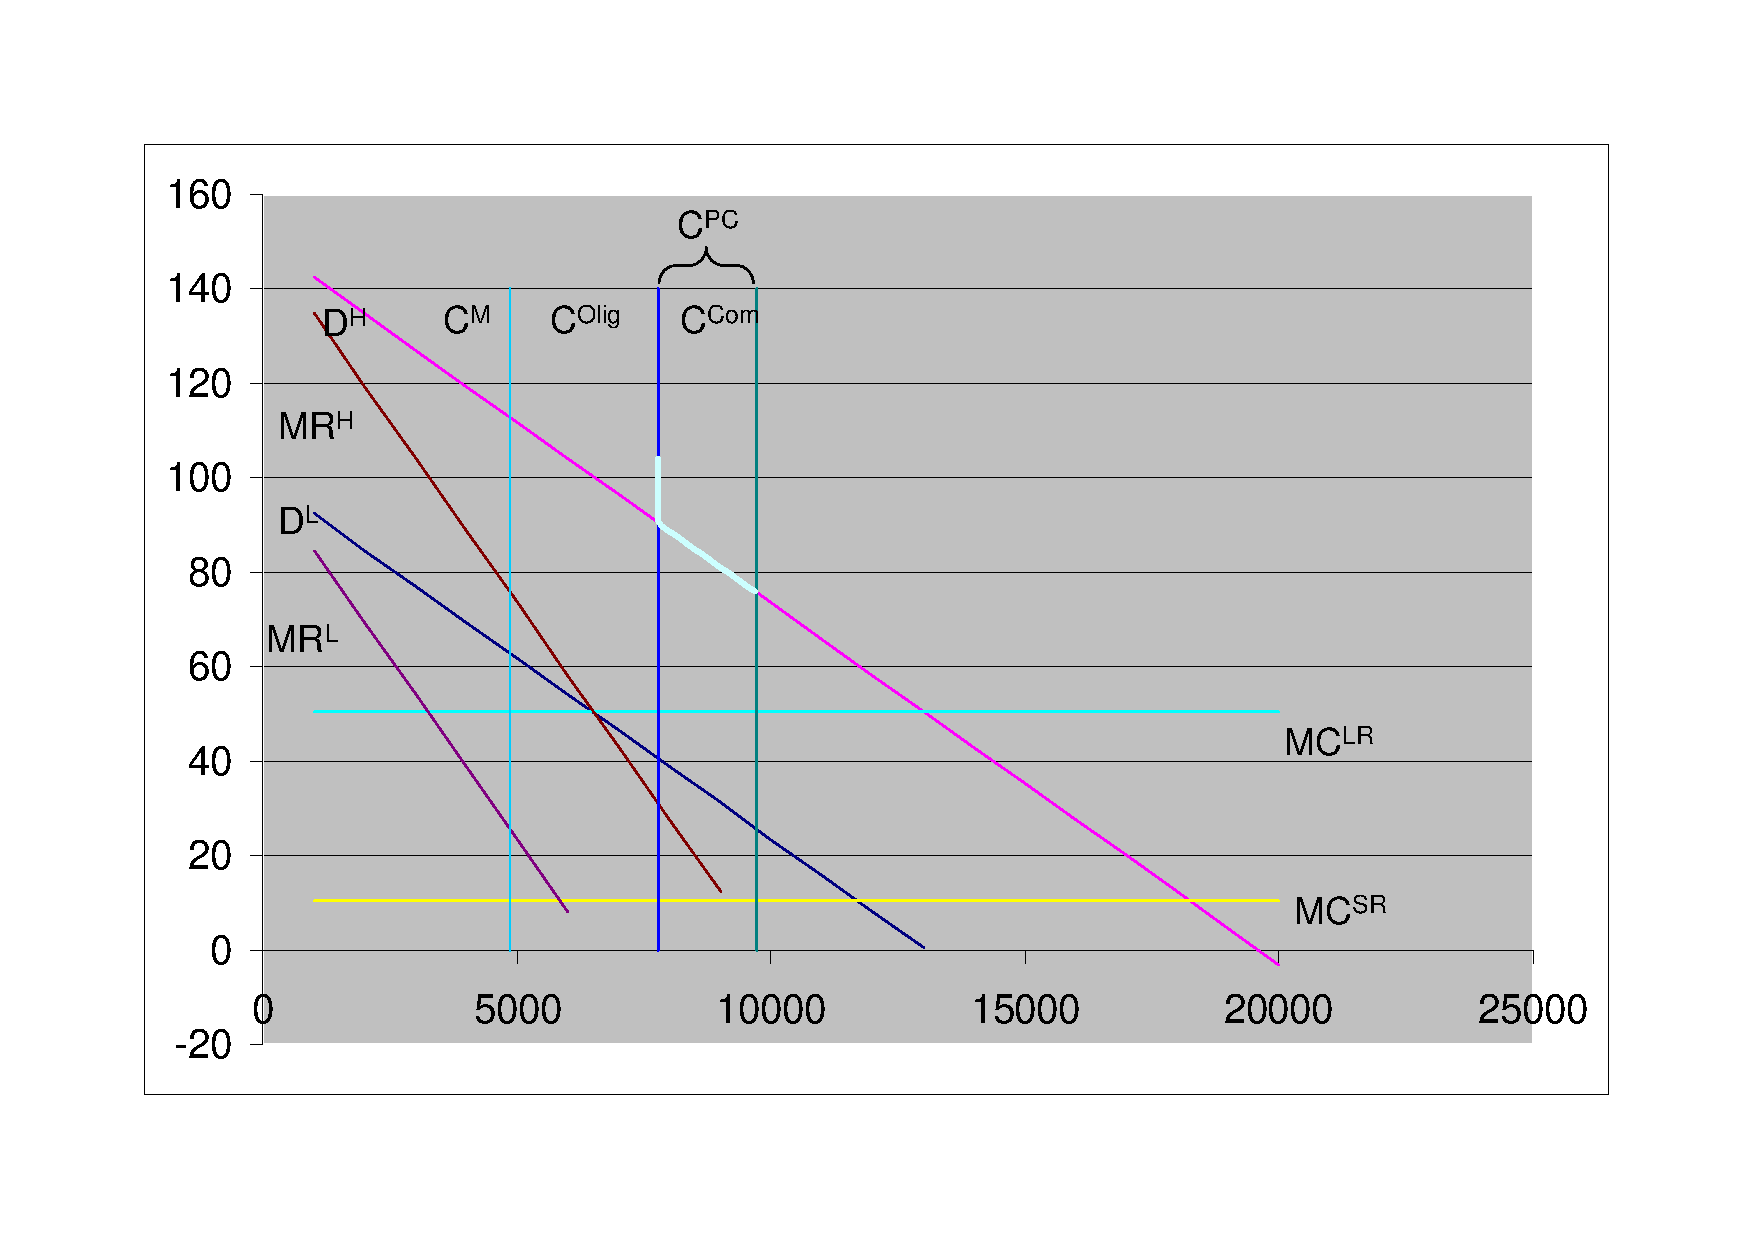
\includegraphics[width=3.0in]{capacity/eigenes_modell}
      \label{eigenes_modell}  
\\          
\scriptsize Source: own calculations
\end{figure}

So under perfect competition, one could rely on the market to provide optimal incentives for capacity investments. However, this does not mean that prices should always be equal to marginal costs, as during peak periods firms must be allowed to cover their investment costs by scarcity rents.

\subsection{Welfare, Options and Capacity Markets}

Following the intuition that scarcity rents are needed to cover investment costs, it is often argued that price caps to mitigate market power destroy investment incentives. The scarcity rents capped by the price cap are generally called the "`missing money"' in the respective stream of Literature over which \cite{Cramton2006} gives an excellent overview.
The same stream of literature argues in favor of capacity markets which should create additional investment incentives. These additional incentives should overcome the missing money problem and seem to be aimed to account for welfare considerations which are not contained into the welfare losses due to rationing which we described above. If capacity is binding, the price of electricity is equal to the willingness to pay of the marginal consumer. The consumers on the electricity wholesale market however, are not the end users but usually retailers and it might well be that they care less than their end users about electricity deliveries which had to be price rationed. A possible solution for this problem might be to make electricity retailers pay penalties for the value of lost load (VOLL). \cite{Burger2007} present a case study case study how this might be done.
An alternative setup is presented in \cite{Boom2007} where a blackout can occur in the case of which all players loose all their rents. \cite{Chao2004} show how market power is mitigated and how new investments are facilitated if option contracts are introduced. We do not account for such market features, although it might be an interesting alternative for further research.
Capacity investments have also been studied from a real option perspective which incorporates the value to delay investments by \cite{Roques2006}.

\subsection{Peak-load pricing under imperfect competition}

The seminal article when it comes to capacity choice under imperfect competition is \cite{Kreps1983} who showed that firms would choose exactly the Cournot quantities in a two stage game. \cite{Gabszewicz1997} analyze investment under demand uncertainty with quantity competition in the second stage and compare that to a Cournot game played in expected demand which they call the Cournot certainty equivalent game. These models are examples of two stage closed loop games. \cite{Grimm2007} uses an analytical closed loop model to analyze the effect of Cournot competition in the first, and Bertrand competition in the second stage for example.
How optimal incentives to invest in electricity generation equipment are distorted by an oligopolistic situation is discussed from a very practical point of view in \cite{Brunekreeft2005} for example. The discussion in \cite{Murphy2005} has been mentioned beforehand already. \cite{Genc2007}, \cite{Genc2007a} and \cite{Lise2008} discuss numerical models of electricity markets based on open loop games but do not focus on economic explanations of the effects found. As we use an open loop information structure, in our model, there is always the same mode of competition in the first and the second stage of the game which might be intuitive, as - at least in the electricity market - there is no obvious reason why firms should first interact on the basis of Cournot and then follow a Bertrand logic or vice versa.
Under imperfect competition, firms might have an incentive to reduce investments, thereby driving up the price in peak periods and increasing their profits. Of course, this only works if there are barriers to entry beyond the unit costs of investment. The effect of lower than optimal investments is depicted in Figure \ref{peak_load_insufficient}.

\begin{figure}[h]
\centering
\caption{Insufficient supply}
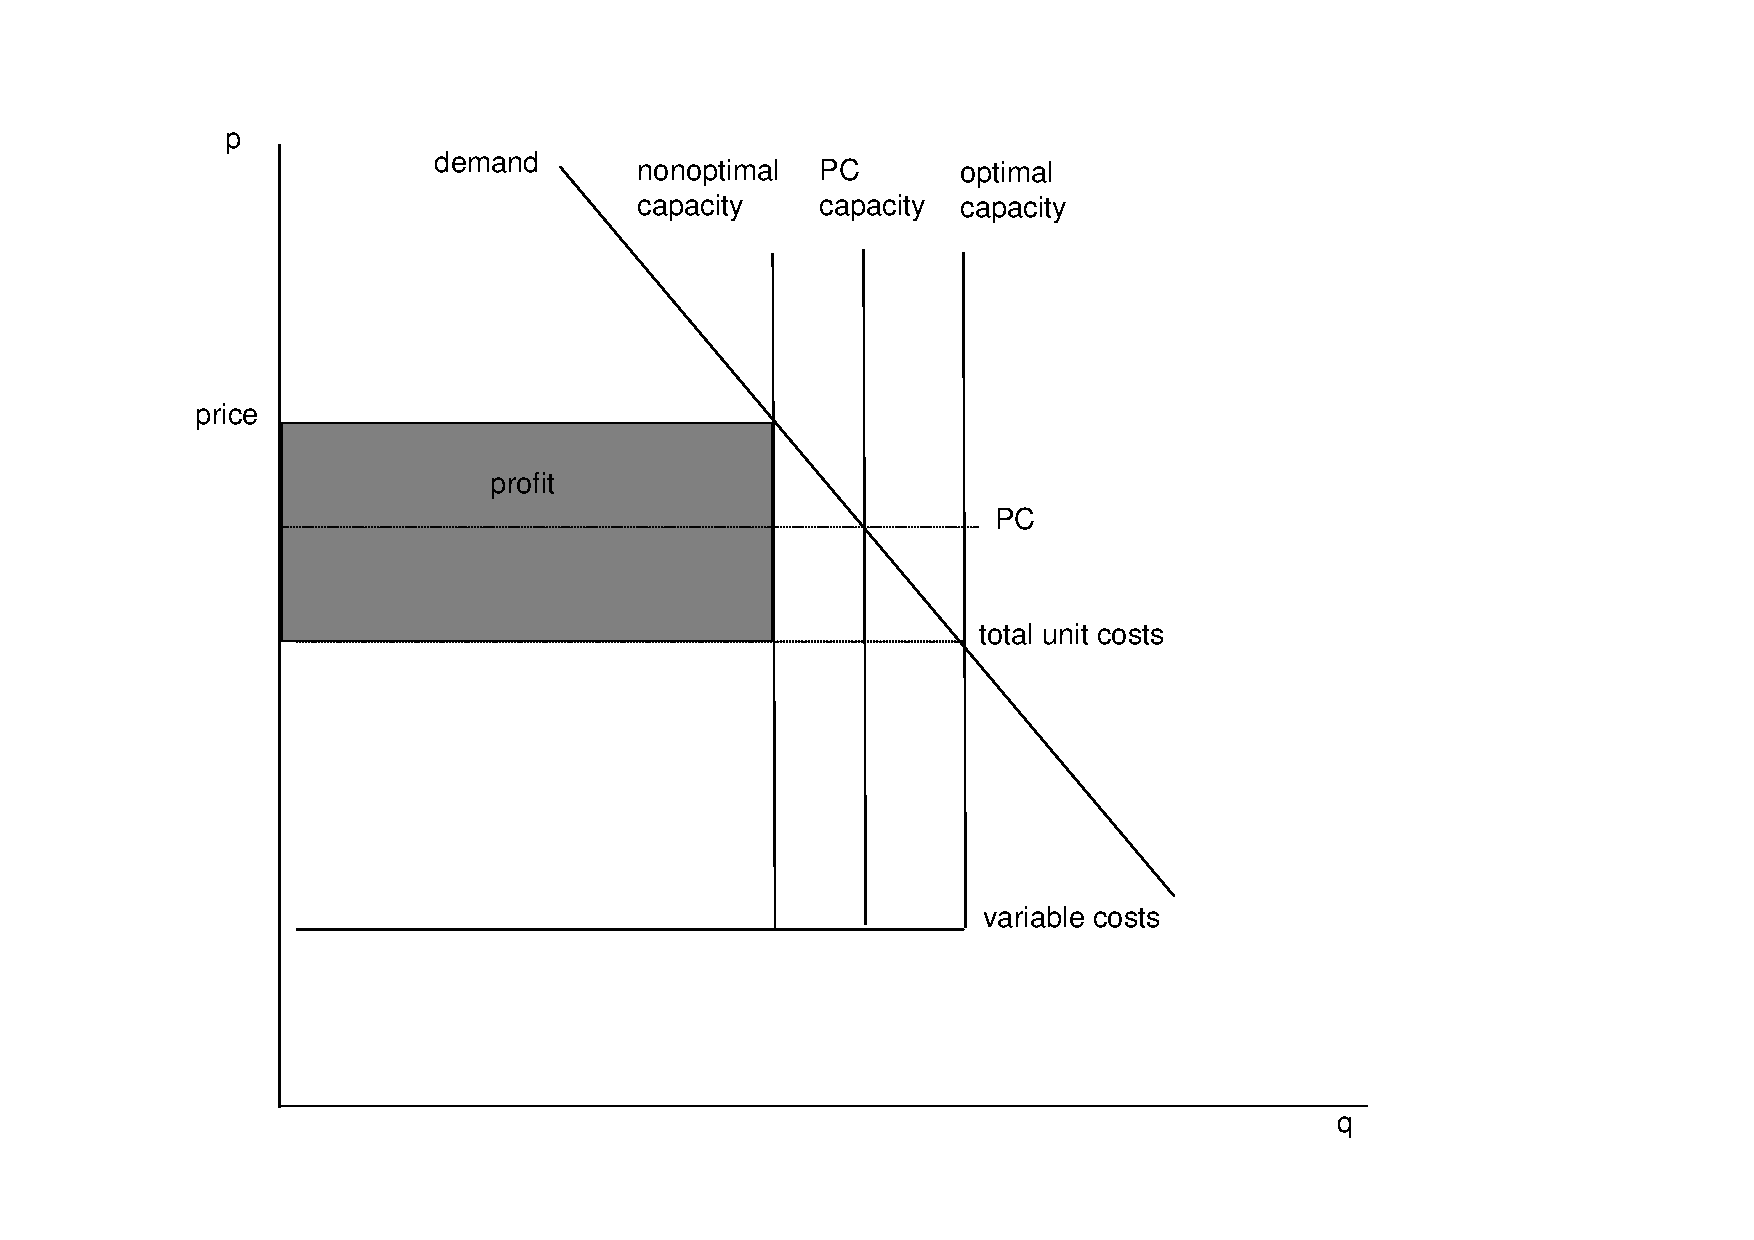
\includegraphics[width=4.2in]{capacity/insufficient_supply.pdf}
      \label{peak_load_insufficient}  
\\          
\scriptsize Source: own calculations
\end{figure}


 
Figure \ref{eigenes_modell} shows results from a simplified version of our model for the Monopoly, Oligopoly (4 Players) and the perfect competition case. It can be seen easily, that there is an underinvestment problem in the case of an oligopoly, which is somewhere between the two benchmark cases. 

%As a monopolist bases it�s decisions on his expected marginal revenue $(MR^H, MR^L)$ Je nachdem wie MR ausssieht erreicht man schneller die - steht am Zettel.

We will now use the example from \cite{Fehr1995} to illustrate the two competing effects.
While the socially optimal incentive to invest is still the same as above, a firm in an oligopolistic situation gets the following expected revenue per unit of investment:

\begin{equation*}
	\frac{1}{2} (1-\pi) (p^{op}-v) + \pi \left(w^p(K)+\frac{\partial w^p(K^*)}{\partial q}-v\right) - c
\end{equation*}

The first part of the equation stands for possible gains of the investment that might occur during low peak periods. For simplicity we assume that there is a duopoly and a probability of $1/2$ for a new unit of capacity to be utilized. This is then multiplied by the probability to not have a peak period $(1-\pi)$ and the oligopoly price minus variable costs $(p^{op}-v)$. In such periods it is possible to steal business, you would normally not have, from another firm. Such an effect can create an additional incentive to invest in capacity. In the case of multiple technologies, a firm could also invest into cheap base load plants which replace plants with higher marginal costs. %As we shall see later on, this effect can be called a strategic effect of investments as well.

The second part of the equation stands for what the investing firm looses in peak periods due to the investment. This equation is essentially the same as the condition we derived for perfect competition. The only difference is that we now write the peak price as a function of the binding capacity $p^p(K)$ and that this price now changes with capacity (and thereby quantity) changes which are illustrated by $\frac{\partial w^p(K^*)}{\partial q}$. This term measures the reduction in the peak price which is due to the decreased scarcity of capacity. This effect has to be taken into account now, as we switched from perfect competition to oligopoly.

So if the loss firms expect due to losses in the peak load market price are bigger than the gains due to more market share in off peak periods, firms will under invest as their incentive to invest is smaller than the optimal level under perfect competition. Of course, if the effect doe to business stealing is higher, firms will overinvest. So in an oligopolistic setting, firms will in general not choose an optimal level of investments.

Figure \ref{peak_load_insufficient} illustrates the effect of a price cap (PC) on investment incentives if the market price is above total unit costs due to market power. The price cap makes it impossible for the firm to increase profits by withholding or not building capacity and thereby, contrary to the missing money argument, can as well increase investments in an oligopolistic setting.

\subsection{Capacity withholding}

What is meant by capacity withholding? In the electricity market context, this term is used to describe a situation in which available capacities are not used even if the price is higher than marginal costs. In a Cournot Situation, capacity withholding naturally occurs in the short run if starting capacities are above the Cournot quantities. Such a situation can be seen in Figure \ref{cournot}. The normal Cournot equilibrium does not satisfy capacity constraints and so a constrained solution evolves from the static game.

\begin{figure}[h]
\centering
\caption{Insufficient supply}
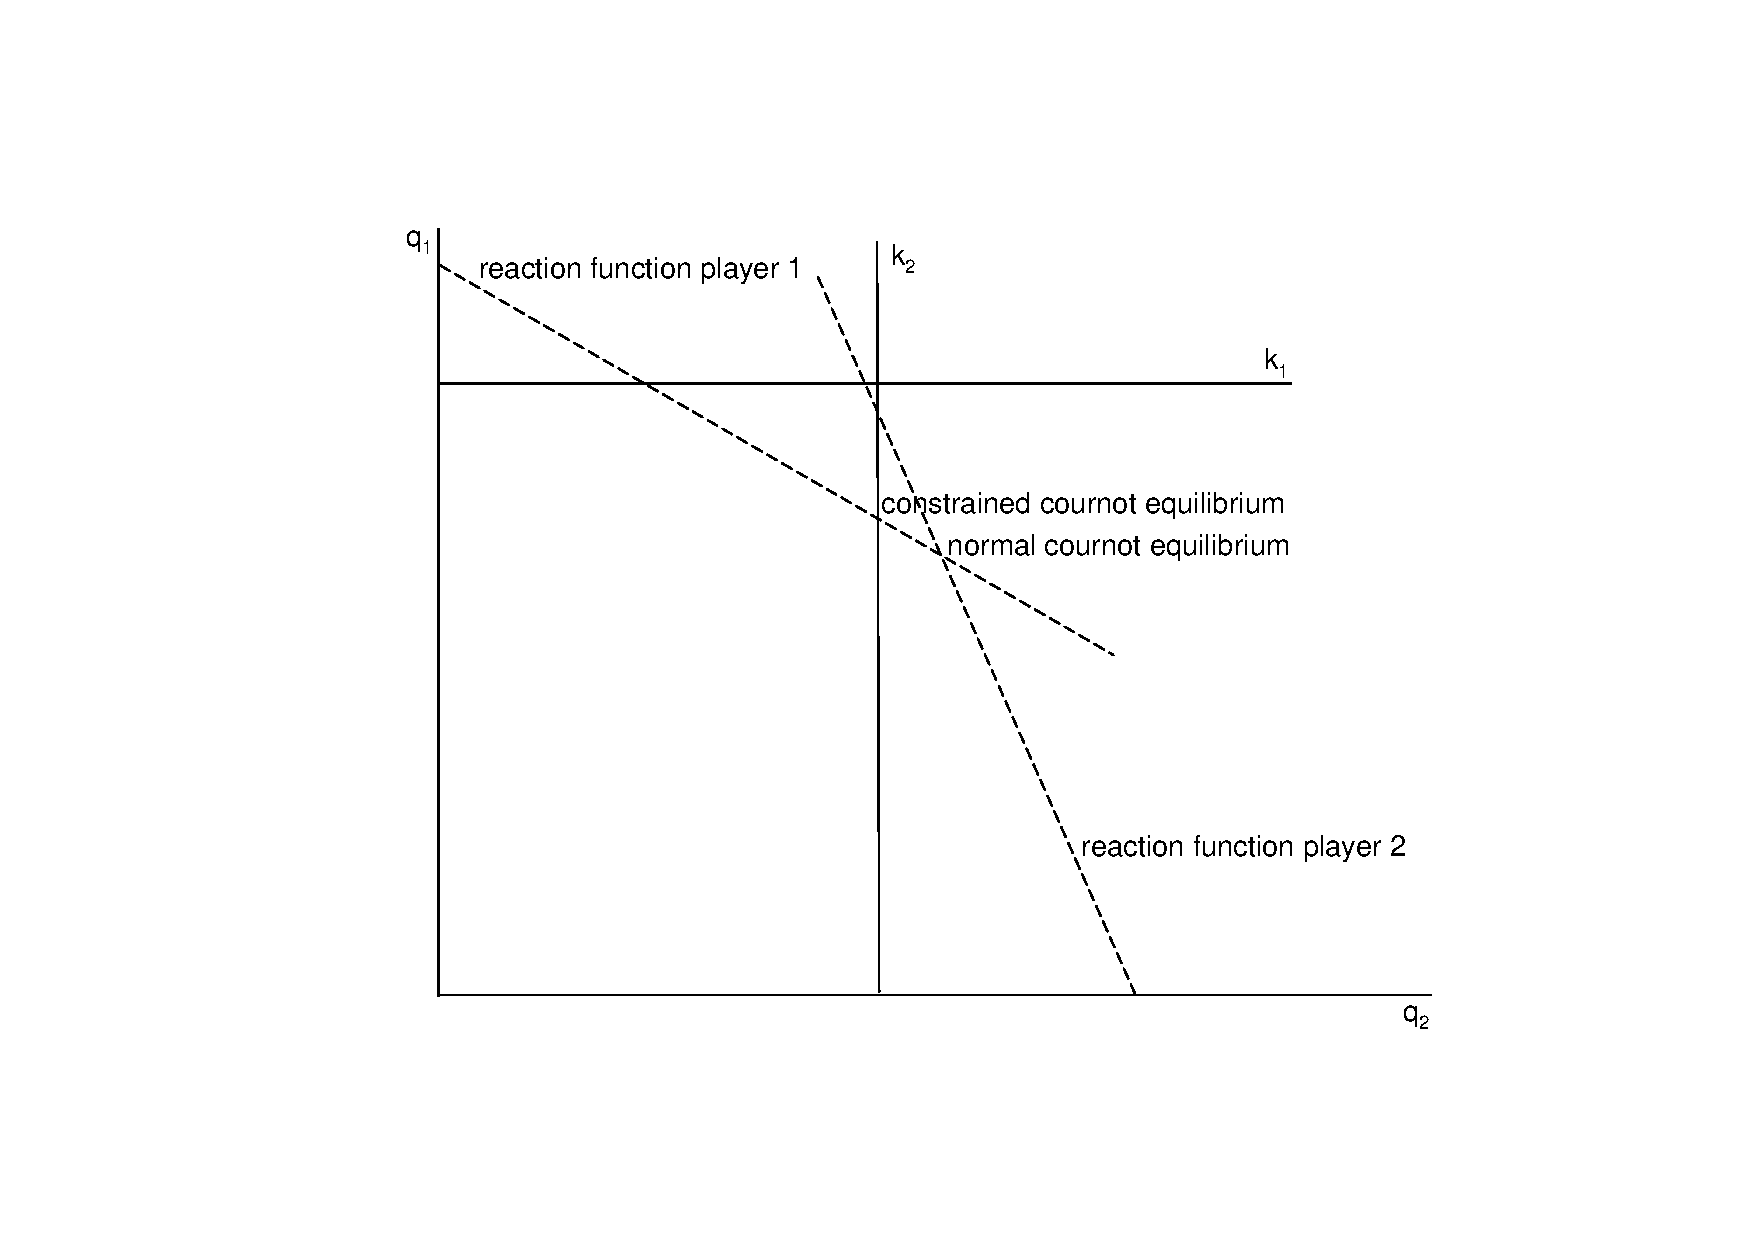
\includegraphics[width=4.2in]{capacity/Cournot.pdf}
      \label{cournot}  
\\          
\scriptsize Source: own calculations
\end{figure}

In a dynamic (open loop??????) setting however, firm one would let his capacity depreciate and firm two would invest until both capacities reach the normal cournot equilibrium. Then, there are no unused capacities any more but capacities itself are not optimal as they resemble an equilibrium with market power. 
If there is uncertainty about future demand there will always by situations with spare capacities. We illustrate this, by considering two different reaction functions, one for high and one for low demand for both players (\ref{cournot_uncertainty}). In such a case, spare capacities in peak periods become unavoidable. Please note that, in this context, uncertainty could resemble different possible loads coming from a load duration curve, or uncertainty about demand growth.

\begin{figure}[h]
\centering
\caption{Insufficient supply}
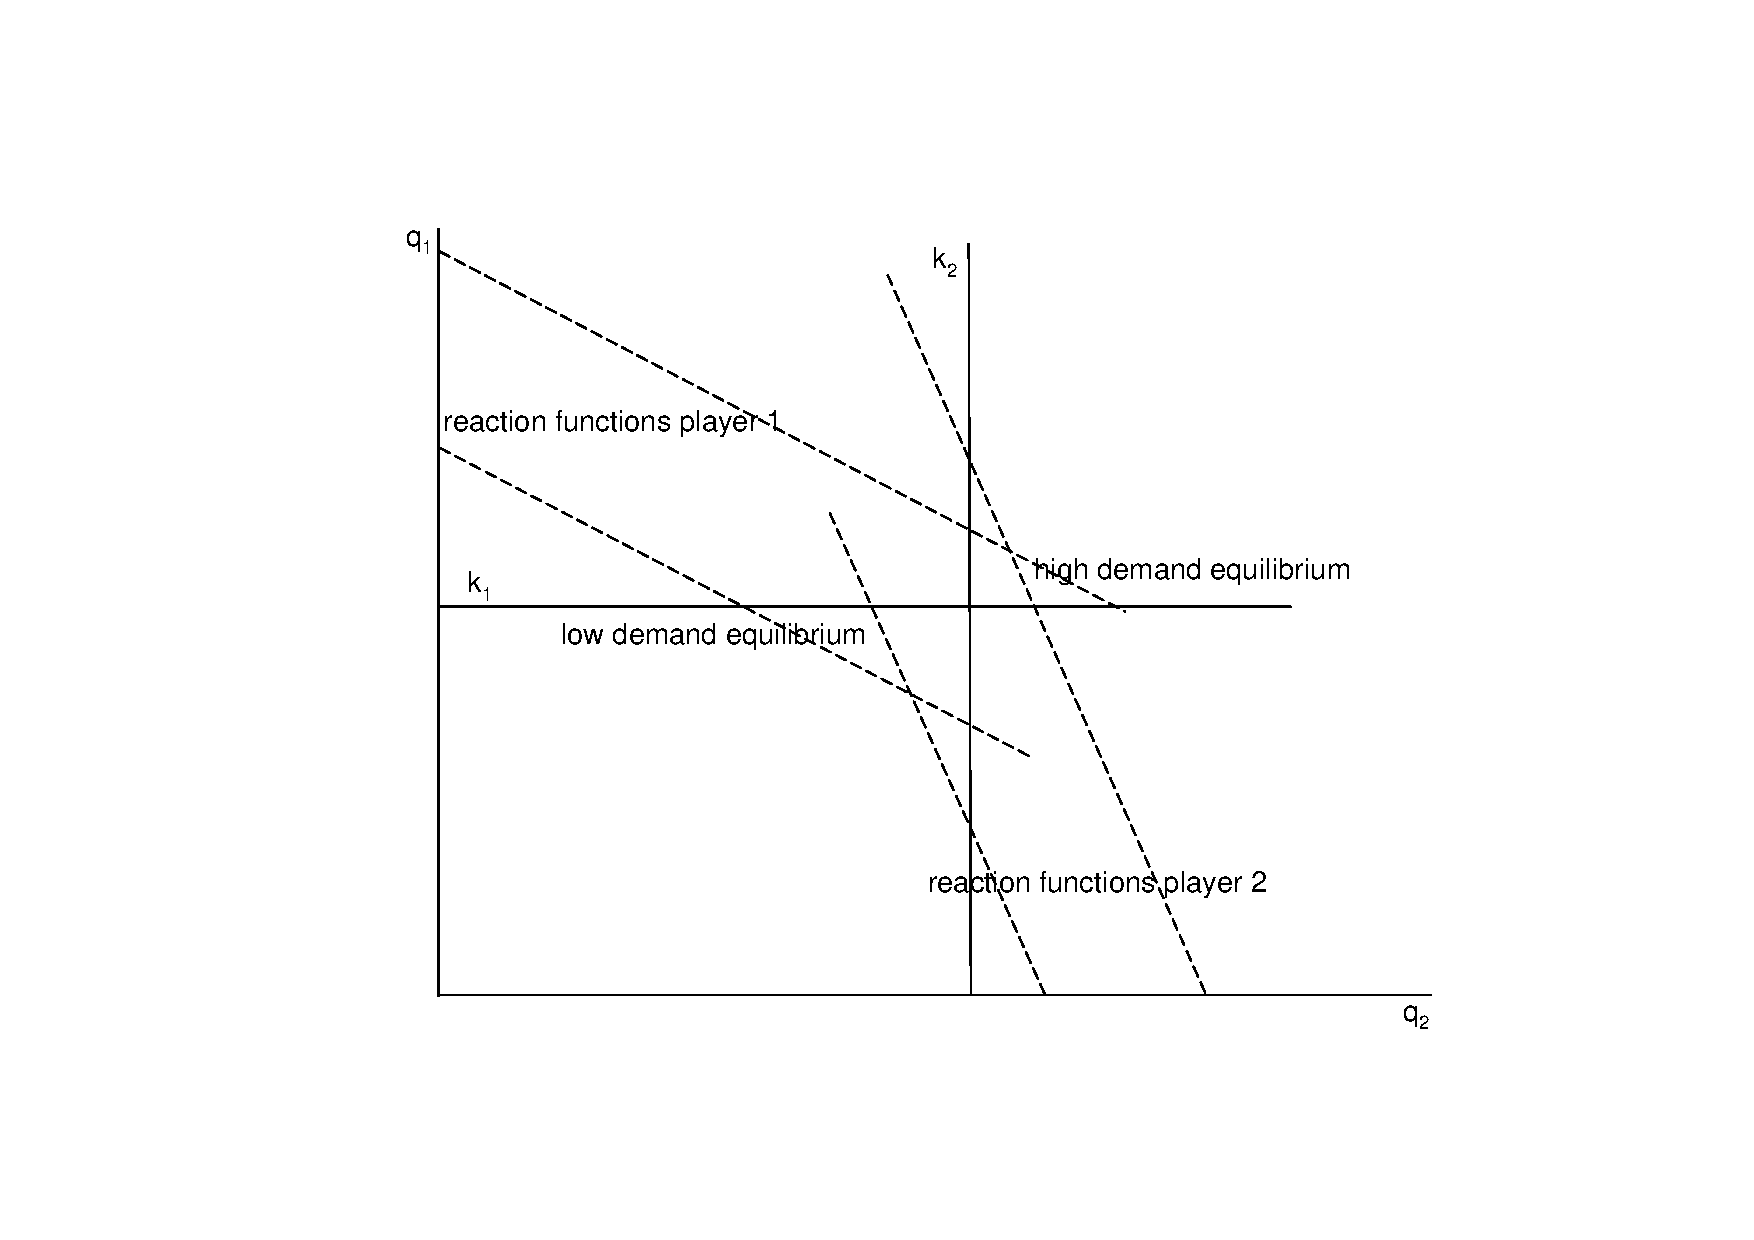
\includegraphics[width=4.2in]{capacity/cournot_uncertainty.pdf}
      \label{cournot_uncertainty}  
\\          
\scriptsize Source: own calculations
\end{figure}

%If there is market power, the above mentioned optimality result does not necessarily hold as prices above marginal costs may induce overinvestments. The situation of too high prices is depicted in Figure \ref{peak_load_toohigh}.

%\begin{figure}[h]
%\centering
%\caption{Imperfectly competitive spot pricing}
%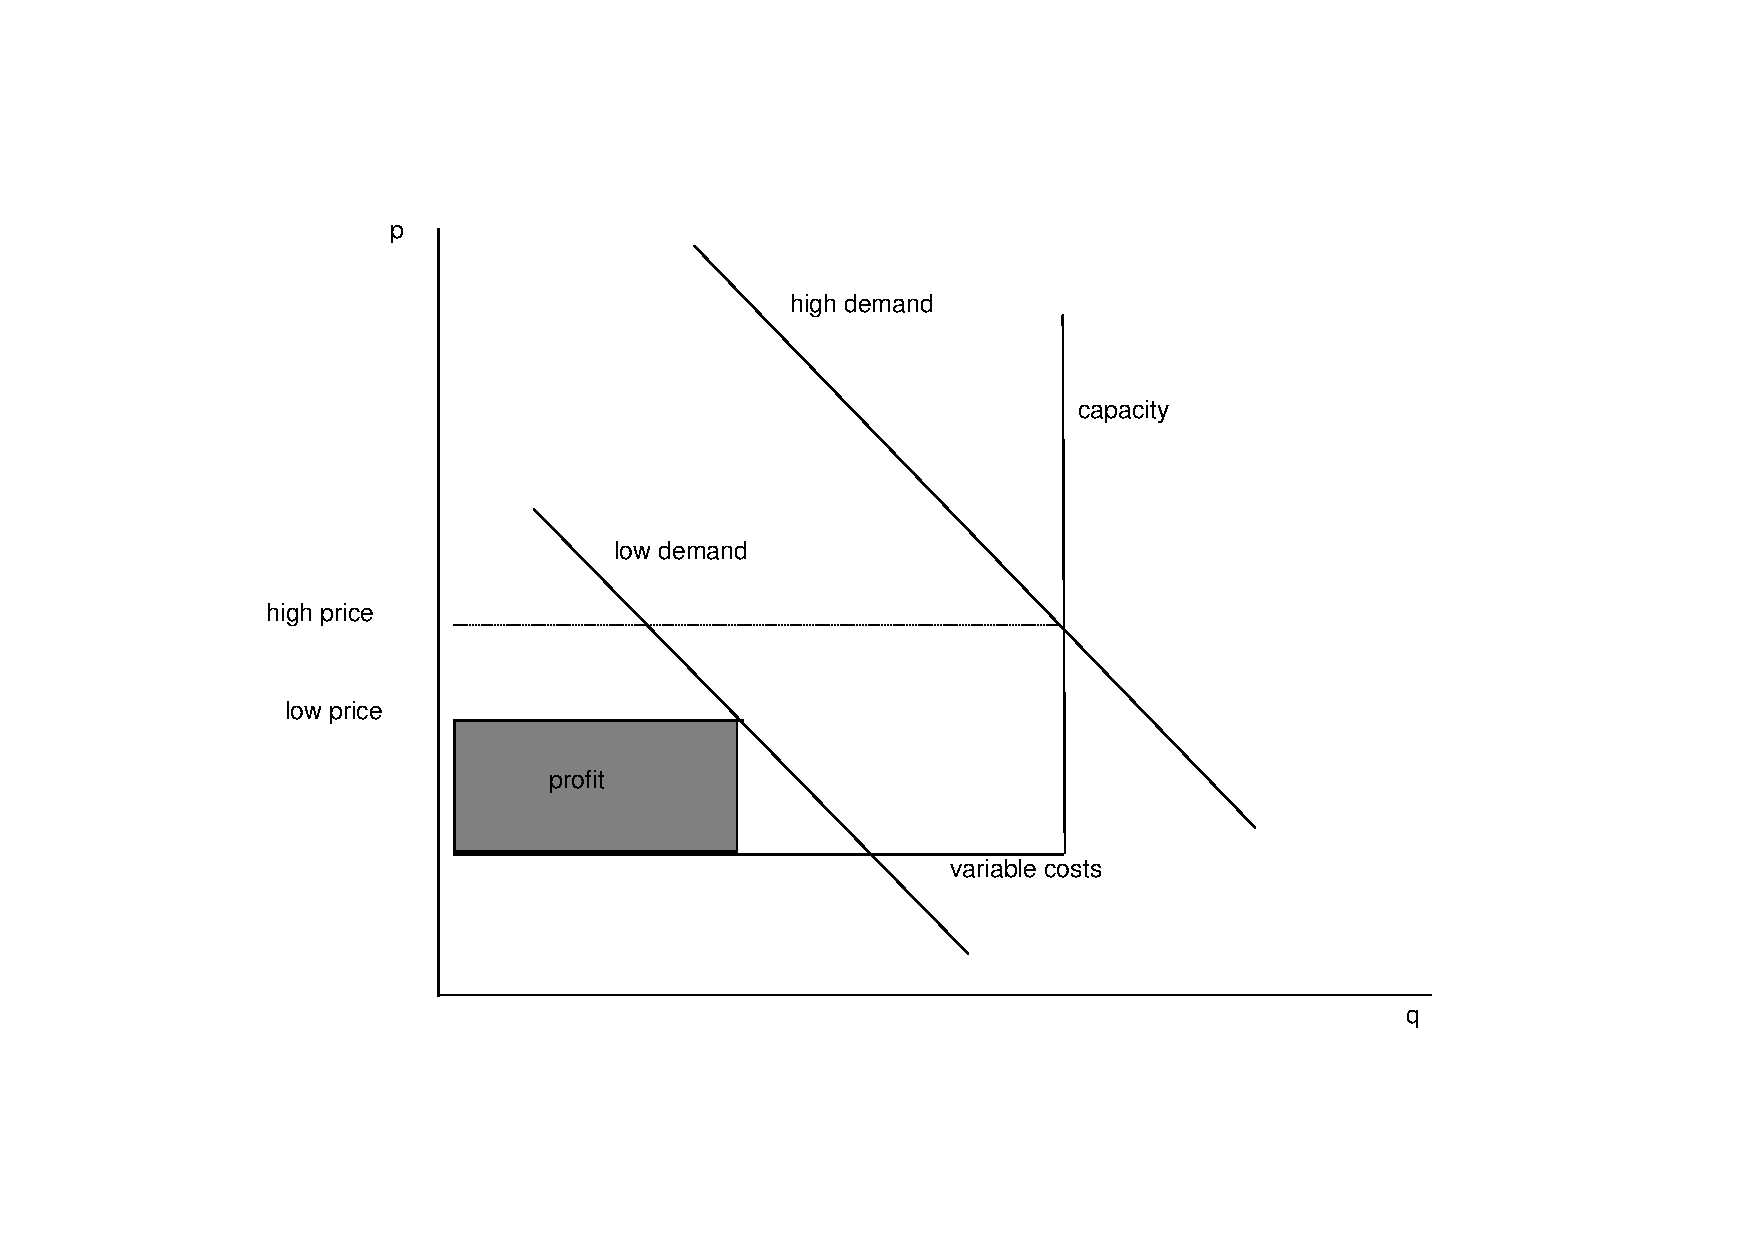
\includegraphics[width=3.0in]{capacity/imperfect_spot_pricing.pdf}
%      \label{peak_load_toohigh}  
%\\          
%\scriptsize Source: \cite{Fehr1995}
%\end{figure}

%The premium of the market price in peak periods ($p^p$) over marginal costs in peak periods, multiplied with the chance of actually having a period of high demand, reflects the value of increasing capacity by one unit.  The value of increasing capacity by one unit must equal capacity costs per unit. If the condition
%$$(p^p-v)\times\pi=c$$
%is met, social surplus is maximized and costs are minimized. A profit maximizing firm under perfect competition would invest until exactly this condition is satisfied. 

%To be able to assess the strength of the different effects, we set up a realistic numerical model in the next section. %As we shall see later on, in a two stage game, strategic effects can be accounted for in different ways which has an effect on the predictions made.

%\subsection{Optimal Technology Mix}

%If demand were certain and constant, only one technology (the one which reaches the lowest possible costs in a standard cost minimization problem with capacity costs and operating costs as inputs) would be used \citep[see][pg. 183]{Chao1983}. This can be seen in the following graph (\ref{technology_choice_chow}) in which a standard cost minimization problem with capacity costs and operating costs as inputs and different technologies are shown. The minimal cost combination given input prices would be technology one. But when demand is uncertain or variable and the output is nonstorable some idle capacity becomes inevitable. This makes less capital intensive technologies such as 2 and 3 more attractive which would be dominated without fluctuations. However, all technologies which are not on the lower envelope are still inferior.

%\begin{figure}[h]
%\centering
%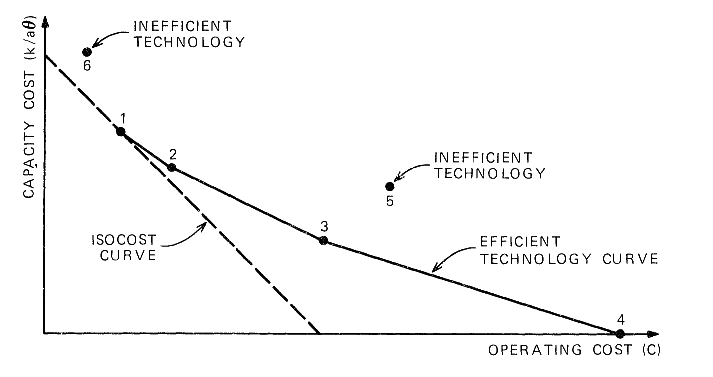
\includegraphics[width=.5\textwidth]{capacity/technology_choice_chow}
%      \label{technology_choice_chow}            
%      \caption{different technologies}
%       source: Chow (1983)
%\end{figure}

%\cite{sherali1982} present a graphical illustration on how to find the optimal mix of different technologies if demand varies. Figure \ref{technology_choice_sherali} \textbf{b} shows the so - called load duration curve which plots the hours of the year ordered according to their energy demand. It can be seen, that only during a few hours of the year demand is very high. Figure \ref{technology_choice_sherali} \textbf{a} shows the cost curves of three different technologies. Technology three has low yearly fixed costs ($c_3$) and high variable costs ($f_3$) so if it would be used for more than $\alpha_{23}$ hours in a year it would be cheaper to use technology two instead. For most of the time of the year, it is actually cheaper to use technology one only which has fairly high fixed but low variable costs. The condition of when one technology becomes cheaper than the other is the same than the one derived by \cite{chow1983} (who also adds an additional stochastic element however). This condition for an optimal technology mix has first been advanced by \cite{Turvey1968}. Also \cite{Pineau2007} uses this condition.

%\begin{eqnarray}
%	c_1 + f_1 \alpha_{12} = c_2 + f_2 \alpha_{12}
%	\alpha_{12} = \frac{c_2-c_1}{f_1-f_2}
%\end{eqnarray}

%This so called optimal running time can be translated into optimal investments into capacity of technology one two and three as can be seen in figure \ref{technology_choice_sherali} \textbf{b}.

%\begin{figure}[h]
%\centering
%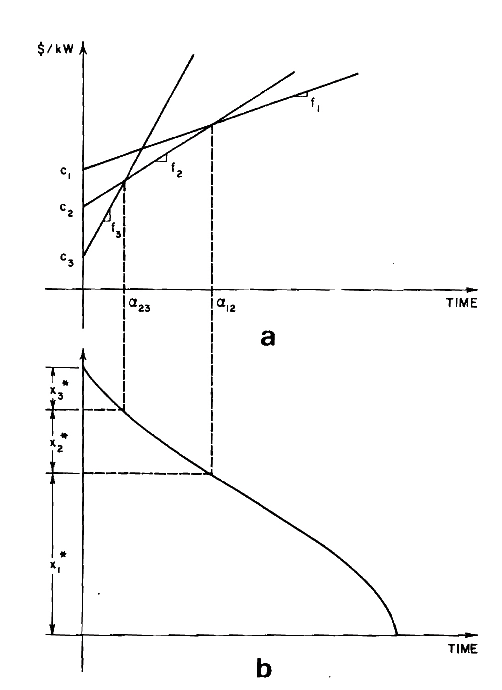
\includegraphics[width=.5\textwidth]{capacity/technology_choice_sherali}
%      \label{technology_choice_sherali}            
%      \caption{the load duration curve and cost curves - graphical determination of the optimal technology mix}
%      source: Sherali et. al. (1982)
%\end{figure}

%What can be seen here is that which kind of capacity is optimal to be built depends on where demand actually increases. It is an unresolved issue whether competition and markets, be it perfect competition or imperfect forms alter the technology mix firms have an incentive to install in any way.



%%% Local Variables: 
%%% mode: latex
%%% TeX-master: "../eem08"
%%% End: 

%\newpage
\section{The model}

\subsection{Static model - peak load pricing}

We begin with a static version of our model to establish the link to the economic intuition outlined in the previous section. There are four players and a strategic fringe, indexed by $i\in N$ (RWE, EON, Vattenfall, EnBW), seven technologies $k\in K$  and six different market states $m\in M$. Each of the players maximizes the following profit function:

\begin{gather}
	\max \pi_i(q_{i,k}^m,K_{i,k},)= \sum_{m\in M} v_m\times\\ \nonumber  \left[(\alpha_m-\beta_m\sum_{i\in N} \sum_{k\in K} q_{i,k}^m ) \sum_{k\in K} q_{i,k}^m - \sum_{k\in K} c^k q_{i,k}^m \right] \\ \nonumber
			\text{s.t.:} \  q_{i,k}^m-K_{i,k} \leq 0;\  \forall i,k,m \\
 										  q_{i,k}^m	\geq 0; \ \forall i,k,m   \nonumber
\end{gather}

\begin{tabular}[c]{l l}
$i\in N$        & players, firms\\
$s\in S$       	& scenarios\\
$m\in M$	& states of the market \\
$k\in K$	& technologies \\
$t\in T$	& time \\
$K_{i,k}^t$      & available capacity at time $t$ from technology $k$ \\
                & for firm $i$ \\
$q_{i,k}^{s,m,t}$ & quantity produced at time $t$ with technology $k$\\
                 &by firm $i$ in market state $m$ and scenario $s$ \\			
$I_{i,k}^t$   & investment in technology $k$ at time $t$  \\
              & by firm $i$\\
$p_s$        & probability of scenario $s$\\
$\nu_m$      & says how often (how many hours) market \\
             & state $m$ occurs \\
$\delta$   & discount factor \\
$\rho$   & depreciation factor \\
$\alpha_m$  & demand function intercept in market state $m$ \\
$\beta_m$   & demand function slope in market state $m$ \\
$c_k$	     & variable costs of technology $k$	\\
$\Gamma_k$   & investment costs in technology $k$  \\
$F_k$        & scrap values  \\
\\
\end{tabular}

$\alpha_m$ and $\beta_m$ are the intercept and the slope of the inverse demand function in the different market states derived from Table \ref{tab:demand}. $q_{i,k}^m$ is the quantity produced with each technology by each player in each market state and $K_{i,k}$ is the corresponding capacity which is now given for each player as we are solving for the short run equilibrium. $c_k$ are the short run variable costs which are the same for each producer. The parameter $\nu_m $ says how often a certain demand state occurs. This parameter is used as a weight for the shadow price of capacity. We derived the Karush Kuhn Tucker (KKT) conditions to obtain a mixed complementarity problem (MCP) and solved it by using the PATH Solver in GAMS.

Table \ref{tab:statquant} in the appendix shows the quantities predicted by our oligopoly model. While during a high demand state almost all capacities are used, during low demand states hard coal plants are the most expensive technology in the merit order curve. Prices differ significantly but are above marginal costs even if demand is very low. Please note, that there is strategic capacity withholding as not all capacities are brought to the market even if more than the variable costs were covered.

As we used a Lagrangian method to calculate this short run equilibrium, we can have a look at the shadow prices of capacity to see how much an additional unit of capacity would be worth for each player. Please note that this values cannot be smaller than zero as, in our setup, there always exists the option of not using existing capacities. There are only positive scarcity rents if the capacity of the technology is binding. So please note that there are positive values for almost all technologies during extremely high demand states as most of the capacities become binding then. \\

Table \ref{tab:statlambda} shows the shadow prices of capacity. The values can be read in such a way that an additional MW of hydro power capacity would increase profits RWE makes in all the extremely high market states by 831 Euros and the overall yearly profit of RWE by 44,832 EUROS. On the contrary, the same capacity is worth 269,972 Euros for EnBW. How can such different results be explained? 

For smaller players like Vattenfall and EnBW shadow prices are far higher as the effect of less scarcity, and thereby lower prices is less important if firms sell less. This means that it is impossible to assess the investment incentives for firms on a market like the electricity market (oligopoly with $L$-shaped cost functions) without considering the strategic implications such investments have.

\subsection{Dynamic model}

In this part, we introduce two deciding factors. First, dynamics and thereby investments which link the different time periods. Second, uncertainty which is accounted for by a binomial scenario tree and leads to a recourse problem. The uncertainty about future demand is accounted for by different demand scenarios. Our approach follows the game with probabilistic scenarios (GPS) method by \cite{Genc2007}. Our two stage Model looks as follows.

\begin{gather}
	\max \pi_i(q_{i,k}^{s,m,t},K^t_{i,k},I_{i,k})=	\\ \nonumber
	\sum_{m\in M} v_m \left[ (\alpha_m^l-\beta_m^l \sum_{i\in N}\sum_{k\in K} q_{i,k}^{l,m,1}) \sum_{k\in K} q_{i,k}^{l,m,1} - \sum_{k\in K} c_k q_{i,k}^{l,m,1} \right]  \\  \nonumber 
	+ \delta \sum_{s\in S} p_s \sum_{m\in M} v_m \times \\ \nonumber \left[ (\alpha_m^s-\beta_m^s \sum_{i\in N}\sum_{k\in K} q_{i,k}^{s,m,2}) \sum_{k\in K} q_{i,k}^{s,m,2} - \sum_{k\in K} c_k q_{i,k}^{s,m,2}  \right]   \\  \nonumber 
									- \sum_{k\in K} \Gamma_{k\in K} I_{i,k} + \delta \sum_{k\in K} F_k I_{i,k}  \\       
			\text{s.t.:} \  q_{i,k}^{l,m,1} - K^{1}_{i,k} \leq 0; \ \forall i,k,m    \label{eq:oligopmax2}\\ 
											q_{i,k}^{s,m,2} - K^{2}_{i,k} \leq 0; \ \forall i,k,m,s  \label{eq:oligopmax3}\\
										  K^{2}_{i,k}  - \rho K^{1}_{i,k}  - I_{i,k} = 0 ; \ \forall i,k  \label{eq:ologopmax5} \\  
 										  q_{i,k}^{s,m,t};K^t_{i,k};I_{i,k}	\geq 0; \ \forall i,k,s   \nonumber
\end{gather}

Each player maximizes its profit by setting $q_{i,k}^{s,m,t}$ and $I_{i,k}^t$. By considering different demand scenarios ($s\in S$) and the associated probabilities ($p_s$), the players take into account how demand might evolve in the future. Capacities now evolve over time $t\in T$ according to the state equation \eqref{eq:ologopmax5}. The capacity constraints are given in \eqref{eq:oligopmax2} and \eqref{eq:oligopmax3}. Quantities are allowed to adapt to the scenarios, thereby accounting for the fact that firms can always react to demand by adjusting their short run production. On the contrary, investments are not allowed to differ in such a way as they have to be set in advance when it is not clear yet how high demand might be. Please note, that quantities do not depend on what other players might invest. They do depend however, on how high own investments are. 
% as the cost function can be changed between period one and two($C^1_i vs. C^2_i$). (Idee - Wenn man das weggibt, m�sste man den Effekt den eigene Investments auf den Marktpreis haben sehen). 
If quantities would depend on investments of other players as well, we would enter the realm of feedback or closed loop games (which are the same in the case of a two-stage game). It has to be noted here that the solution of a closed loop game can, and will, in general, be different from the solution of an open loop game.

In an alternative version of our model, we implemented a Price Cap ($PC$), so the following additional constraint was added:

\begin{gather}
(\alpha_m^s-\beta_m^s \sum_{i\in N}\sum_{k\in K} q_{i,k}^{s,m,t}) - PC \leq 0; \ \forall s,m
\end{gather}

Adding price caps showed interesting results as investments indeed seemed to increase when price caps were lowered. As this is work in progress however, the results are not given jet. \\

To solve the model, we derive the KKT conditions to obtain an MCP problem which we solve by using GAMS and the PATH solver. For the model above, we used the Cournot approach to derive the first order conditions\footnote{Apart from the strategic fringe, which is assumed to be a price taker.}. For the competitive benchmark, we solved the problem under the assumption that just one welfare maximizing player disposes of all the initial capacities of the five players. The welfare maximizing player is assumed to set prices equal to marginal costs.



%\clearpage




%%% Local Variables: 
%%% mode: latex
%%% TeX-master: "../eem08"
%%% End: 

\section{Results} 

In this first version of the model with only two stages we considered a framework in which firms decide upon investments now, and the second stage of the game lasts for five years. For the discount factor, we assume an interest rate of 3\% and thereby assume that this figure is the same for all players. Equivalently, we set the depreciation rate to 3\% a year. Our setup is such that we can answer to what extent, in the medium run, investment paths that arise from our oligopolistic market deviate from the optimum. In stage zero, the results are the same as in the static version of our model (table \ref{tab:statquant}). For the investment incentive, now expected shadow prices (by considering the different demand scenarios that might evolve) are considered by the firms when they decide whether and in which technology to invest in.

\begin{table}
\centering
\caption{Comparison of optimal vs. oligopoly results in different times and scenarios}
% Table generated by Excel2LaTeX from sheet 'Tabelle1'
% Table generated by Excel2LaTeX from sheet 'Tabelle1'
% Table generated by Excel2LaTeX from sheet 'Tabelle1'
% Table generated by Excel2LaTeX from sheet 'Tabelle1'
\begin{tabular}{llrrrrrr}
\hline
\hline
           &            &    exthigh &      vhigh &       high &      inter &        low &       vlow \\
\hline
     t = 0 &            &            &            &            &            &            &            \\
\hline
 olig. &          q &     72,863 &     69,580 &     66,698 &     61,660 &     49,427 &     34,847 \\

           &          p &        210 &        149 &        118 &         83 &         52 &         27 \\
\hline
   opt. &          q &     82,498 &     82,498 &     77,344 &     73,331 &     63,273 &     41,546 \\

           &          p &        136 &         81 &         72 &         44 &         17 &         16 \\
\hline
\hline
     t = 1 &            &            &            &            &            &            &            \\

 olig. &            &            &            &            &            &            &            \\

       low &          q &     75,922 &     72,898 &     70,468 &     65,094 &     52,295 &     35,817 \\

           &          p &        186 &        132 &        102 &         72 &         45 &         26 \\

      high &          q &     79,105 &     76,176 &     72,864 &     67,972 &     54,711 &     37,861 \\

           &          p &        200 &        140 &        112 &         77 &         48 &         26 \\
\hline
   opt. &            &            &            &            &            &            &            \\
       low &          q &     94,509 &     91,497 &     86,167 &     81,578 &     65,952 &     44,771 \\
           &          p &         44 &         34 &         34 &         16 &         11 &         11 \\
           &            &            &            &            &            &            &            \\
      high &          q &     96,839 &     94,397 &     90,860 &     84,879 &     67,284 &     47,327 \\
           &          p &         65 &         44 &         34 &         20 &         16 &         11 \\
\hline
\hline
\end{tabular}  

\label{tab:dynquant}
\begin{center}
source: own calculations
\end{center}
\end{table}

Total quantities and prices for the oligopoly model and the perfectly competitive model at each point in time, and each scenario are given in table \ref{tab:dynquant}. Of course, prices are lower in the low demand scenarios than in the high demand scenarios. However, in all cases, due to investments and thereby higher quantities, prices in period one are lower than in period zero.
Compared to the optimal results for prices and qualities, prices are always higher and quantities are lower in the oligopoly case.

Our main results are our predictions for invested quantities. It can be seen in table \ref{tab:invest} that, given the cost and demand information we have, brown coal seems to be the dominant technology choice. If we rule out brown coal, which might be plausible as there is only a limited number of available sites, nuclear plants for the social planner, and nuclear and hard coal plants for the oligopolists become the technology of choice as can be seen in table \ref{tab:invest}.

What can be said without ambiguity, is that the amount of capacity which is built is considerably distorted downwards by the effects of oligopolistic competition in an otherwise unchanged model. For most of the players, additional capacity is of no value, even in high demand states. This is intuitive however, as an additional unit of capacity might be not worth it for a big player because it lowers the price he gets for all the other units sold. For small players like Vattenfall and EnbW an additional unit of capacity is of more value, at least in high market states. Additionally, is seems that imperfect competition distorts investment choices away from flexible but capital intensive technologies.

\begin{table}
\centering
\caption{Investments in different market forms, with and without availability of B. Coal sites (MW)}
% Table generated by Excel2LaTeX from sheet 'Tabelle1'
\begin{tabular}{llrrrr}
\hline
\hline
investments &            &            &            & \multicolumn{ 2}{r}{Scen. w. Brown Coal} \\
\hline
 oligopoly &            & Brown Coal &            &    Nuclear &  Hard Coal \\
\hline
           &        EON &       1063 &            &            &            \\
           &     Vatten &       7256 &            &       6249 &        283 \\
           &       EnBW &       9102 &            &       8248 &            \\
           &        Sum &      17422 &            & \multicolumn{ 2}{c}{14780} \\
\hline
   optimum &            &      31096 &            &      27658 &            \\
\hline
\hline
\end{tabular}  

\label{tab:invest}
\begin{center}
source: own calculations
\end{center}
\end{table}

\section{Conclusions}

In this paper, we investigate inhowfar deregulated electricity markets can be expected to deliver optimal capacity investments. A purely analytical model cannot answer this question as, from the analytical side, as pointed out in Section \ref{sect:3}, it is unclear whether the combination of a peak load pricing problem, an oligopolistic market structure and uncertainty will create under- or even overinvestment. The German electricity market provided us with a real world example for our numerical model. Building on \cite{Genc2007} we extend their framework further toward a more realistic representation of market states and technologies and develop a normative welfare-optimal benchmark. We came to the preliminary conclusion that there seems to be an underinvestment problem arising from the current market framework. Additionally, it seems as if the current market setup distorts investment choices away from flexible but capital intensive technologies. This conclusion looks even gloomier in the light of aging plants which have to be replaced and the nuclear phase out.

Further research will focus on a model which allows more conclusions about the long run development of capacities. Additionally, the use of different information structures would be interesting.



%%% Local Variables: 
%%% mode: latex
%%% TeX-master: "../emarket_simulation"
%%% End: 
 

%\section{Ideas}

\begin{itemize}
	\item \cite{Pineau2003} study how electricity prices, production levels and production capacities unfold in \emph{absence of regulation}. Why test different regulatory measures in this game theoretic setting?
	\item Can transmission pricing and constraints also be ignored in Austria?
	\item Parameters to check in sensitivity analysis: depreciation rate of generating capacity
\end{itemize}



%------------------------------------------------------

\markboth{References}{References} %\frenchspacing
\bibliographystyle{chicago}
%\nocite{*}
\bibliography{microsim}

\appendix
\newpage
\section*{Appendix}
%\begin{landscape}

\begin{table}
\scriptsize
\begin{tabular}[h]{ccccc}
\hline
\textbf{Investment problem}\\
\hline
  Authors & Information structure & Solution method & Transmission network & Numerical application \\
\hline
\cite{Genc2007} & $S$-adapted open-loop & MCP & No & electricity market, Ontario, Canada\\
1 & 2 & 3 & 4 & 5 \\
\hline
\textbf{Stochastic oligopoly models}\\
\hline
\cite{Salant1982}\\
\cite{Wolf1997}\\
\cite{Haurie2001}\\
\cite{Haurie2002}\\
\cite{Murto2004}
\end{tabular}
\end{table}
bla ble blu


\textbf{References:} \cite{Salant1982, Wolf1997, Haurie2001, Haurie2002, Pineau2003, Murto2004}\\


The $S$-adapted information structure was introduced by \cite{Haurie1990}.
$S$-adapted structure is similar to the open-loop case, except that the strategies of the players adapt to the sample path of the stochastic variable \citep[see][pg. 128]{Pineau2003}.

\cite{Haurie2002} developed an approximation method with variational inequalities for $S$-adapted oligopoly equilibria. It can be used with any discrete state process that can be represented as an event tree can be used as description of the random disturbances.

\cite{Murto2004} solves the game with feedback information structure.

\cite{Haurie2001}, \cite{Genc2007}

developed an approximation method with variational inequalities for $S$-adapted oligopoly equilibria. It can be used with any discrete state process that can be represented as an event tree can be used as description of the random disturbances.


Market simulation: \cite{Torre2003}, \cite{Valenzuela2007}, \cite{Hobbs2001},\cite{Otero-Novas2000}

General review paper: \cite{Neuhoff2005}, \cite{Ventosa2005}, \cite{Kahn1998}

\end{landscape}



%%% Local Variables: 
%%% mode: latex
%%% TeX-master: "../emarket_simulation"
%%% End: 


\begin{table}[htb]
\centering
\caption{quantities offered and market prices by different firms in different market states}
% Table generated by Excel2LaTeX from sheet 'Tabelle1'
\begin{tabular}{llrrrrrr}
\hline
\hline
           &            & extr. high &    v. high &       high &    interm. &        low &     v. low \\
\hline
       RWE & Hydro Power &        741 &        741 &        741 &        741 &        741 &        741 \\

           &    Nuclear &       5499 &       5499 &       5499 &       5499 &       5499 &       5499 \\

           &    Lignite &      10554 &      10554 &      10554 &      10554 &      10285 &       3684 \\

           &  Hard Coal &       7249 &       7249 &       6675 &       3124 &            &            \\

           &  {\bf Sum} & {\bf 24043} & {\bf 24043} & {\bf 23469} & {\bf 19918} & {\bf 16525} & {\bf 9924} \\
\hline
       EON & Hydro Power &       1320 &       1320 &       1320 &       1320 &       1320 &       1320 \\

           &    Nuclear &       8473 &       8473 &       8473 &       8473 &       8473 &       8473 \\

           &    Lignite &       1425 &       1425 &       1425 &       1425 &       1425 &        131 \\

           &  Hard Coal &       9461 &       9461 &       9461 &       8700 &       3133 &            \\

           &        Gas &       2340 &       1238 &            &            &            &            \\

           &  {\bf Sum} & {\bf 23019} & {\bf 21917} & {\bf 20679} & {\bf 19918} & {\bf 14351} & {\bf 9924} \\
\hline
Vattenfall & Hydro Power &          9 &          9 &          9 &          9 &          9 &          9 \\

           &    Nuclear &       1421 &       1421 &       1421 &       1421 &       1421 &       1421 \\

           &    Lignite &       6932 &       6932 &       6932 &       6932 &       6932 &       6932 \\

           &  Hard Coal &       1729 &       1729 &       1729 &       1729 &       1729 &            \\

           &        Gas &        870 &        870 &        870 &        870 &            &            \\

           &        Oil &       1429 &       1429 &       1429 &        702 &            &            \\

           &   Pump St. &       2883 &        702 &            &            &            &            \\

           &  {\bf Sum} & {\bf 15273} & {\bf 13092} & {\bf 12390} & {\bf 11663} & {\bf 10091} & {\bf 8362} \\
\hline
      EnBW & Hydro Power &        447 &        447 &        447 &        447 &        447 &        447 \\

           &    Nuclear &       4272 &       4272 &       4272 &       4272 &       4272 &       4272 \\

           &    Lignite &        453 &        453 &        453 &        453 &        453 &        453 \\

           &  Hard Coal &       3288 &       3288 &       3288 &       3288 &       3288 &       1465 \\

           &        Gas &       1083 &       1083 &       1083 &       1083 &            &            \\

           &        Oil &        617 &        617 &        617 &        617 &            &            \\

           &   Pump St. &        368 &        368 &            &            &            &            \\

           &  {\bf Sum} & {\bf 10528} & {\bf 10528} & {\bf 10160} & {\bf 10160} & {\bf 8460} & {\bf 6637} \\
\hline
           &    ov. Sum & {\bf 72863} & {\bf 69580} & {\bf 66698} & {\bf 61660} & {\bf 49427} & {\bf 34847} \\
\hline
           &      Price &  {\bf 210} &  {\bf 149} &  {\bf 118} &   {\bf 83} &   {\bf 52} &   {\bf 27} \\
\hline
\hline
\end{tabular}
\label{tab:statquant}
\begin{center}
Source: own calculations
\end{center}
\end{table}

\clearpage
\newpage
%\vspace{3cm}
\begin{table}[htb]
\centering
\caption{shadow prices of capacity, separated by technologies and market states}
% Table generated by Excel2LaTeX from sheet 'Tabelle1'
\begin{tabular}{llrrrrrrr}
\hline
           &            & extr. high &    v. high &       high &    interm. &        low &     v. low &  {\bf Sum} \\
\hline
       RWE & Hydro Power &        831 &       1970 &       6698 &      18479 &      12603 &       4251 & {\bf 44832} \\

           &    Nuclear &        743 &       1715 &       5201 &      14348 &       4621 &       1559 & {\bf 28188} \\

           &    Lignite &        693 &       1568 &       4334 &      11957 &            &            & {\bf 18552} \\

           &  Hard Coal &        440 &        831 &            &            &            &            & {\bf 1271} \\
\hline
       EON & Hydro Power &       1191 &       3471 &      16261 &      18479 &      35709 &       4251 & {\bf 79362} \\

           &    Nuclear &       1104 &       3216 &      14764 &      14348 &      27727 &       1559 & {\bf 62718} \\

           &    Lignite &       1053 &       3069 &      13897 &      11957 &      23106 &            & {\bf 53082} \\

           &  Hard Coal &        800 &       2332 &       9563 &            &            &            & {\bf 12695} \\
\hline
Vattenfall & Hydro Power &       3917 &       9702 &      44668 &      79134 &      81002 &       7954 & {\bf 226377} \\

           &    Nuclear &       3830 &       9447 &      43171 &      75003 &      73020 &       5262 & {\bf 209733} \\

           &    Lignite &       3779 &       9300 &      42304 &      72612 &      68399 &       3703 & {\bf 200097} \\

           &  Hard Coal &       3526 &       8563 &      37970 &      60655 &      45293 &            & {\bf 156007} \\

           &        Gas &       2726 &       6231 &      24259 &      22827 &            &            & {\bf 56043} \\

           &        Oil &       2243 &       4824 &      15985 &            &            &            & {\bf 23052} \\

           &   Pump St. &        587 &            &            &            &            &            &  {\bf 587} \\
\hline
      EnBW & Hydro Power &       5587 &      11512 &      52311 &      90176 &      98341 &      12045 & {\bf 269972} \\

           &    Nuclear &       5500 &      11257 &      50814 &      86045 &      90359 &       9352 & {\bf 253328} \\

           &    Lignite &       5449 &      11110 &      49947 &      83654 &      85738 &       7794 & {\bf 243692} \\

           &  Hard Coal &       5196 &      10373 &      45613 &      71697 &      62633 &            & {\bf 195512} \\

           &        Gas &       4396 &       8041 &      31902 &      33869 &            &            & {\bf 78208} \\

           &        Oil &       3913 &       6634 &      23628 &      11042 &            &            & {\bf 45217} \\

           &   Pump St. &       2257 &       1810 &            &            &            &            & {\bf 4067} \\
\hline
\hline
\end{tabular}  
\label{tab:statlambda}
\begin{center}
Source: own calculations
\end{center}
\end{table}
\end{document}

%%% Local Variables: 
%%% mode: latex
%%% TeX-master: t
%%% End: 
